\documentclass[10pt, aspectratio=169]{beamer}
\usepackage[italian]{babel}
\usepackage[utf8]{inputenc}

\usepackage{graphicx}
\usepackage{amsmath,amssymb}
\usepackage{url} 
\usepackage{comment}
\usepackage{booktabs}
\usepackage{url}
\usepackage{listings}
\lstset{breakatwhitespace,
	language=C++,
	columns=fullflexible,
	keepspaces,
	breaklines,
	tabsize=3, 
	showstringspaces=false,
	extendedchars=true}


\usepackage{graphicx}
\title{Qt: Introduzione al framework}
\subtitle{}
\author{Daniele Liciotti}
\institute{ICT Engineer and PhD Student}
% logo of my university
\titlegraphic{
\includegraphics[width=2.5cm]{images/fermolug-logo.png}
	\hspace{3cm}
	
\includegraphics[width=2.1cm]{images/linuxday-logo.png}
}
\date{Fermo, 24 Ottobre, 2015}
\subject{LinuxDay2015}

\usetheme{Luebeck}
\usecolortheme{crane}

%\useoutertheme{infolines}

\defbeamertemplate*{footline}{infolines}
{
  \leavevmode%
  \hbox{%
  \begin{beamercolorbox}[wd=.333333\paperwidth,ht=2.25ex,dp=1ex,center]{author in head/foot}%
    \usebeamerfont{author in head/foot}\insertshortauthor
  \end{beamercolorbox}%
  \begin{beamercolorbox}[wd=.333333\paperwidth,ht=2.25ex,dp=1ex,center]{title in head/foot}%
    \usebeamerfont{title in head/foot}\insertshorttitle
  \end{beamercolorbox}%
  \begin{beamercolorbox}[wd=.333333\paperwidth,ht=2.25ex,dp=1ex,right]{date in head/foot}%
    \usebeamerfont{date in head/foot}\insertshortdate{}\hspace*{2em}
    \insertframenumber{} / \inserttotalframenumber\hspace*{2ex} 
  \end{beamercolorbox}}%
  \vskip0pt%
}


\begin{document}
\maketitle
\begin{frame}
	\begin{block}{\textbf{Daniele Liciotti}}
		\begin{columns}
			\column{0.6\textwidth}
			\vspace{1cm}\\
			\emph{Ph.D. Student}\\
			Università Politecnica delle Marche\\
			Dipartimento di Ingegneria dell'Informazione\\
			
			\vspace{1cm}
			e-mail:\qquad \emph{danielelic@gmail.com}
			\column{0.3\textwidth}
			\begin{figure}
				\centering
				
\includegraphics[height=3cm]{images/me.png}
			\end{figure}
		\end{columns}
	\end{block}
\end{frame}

\begin{frame}{Un po di storia}
	\begin{itemize}
		\item 1991 si iniziò a scrivere le prime classi di Qt
		\item 1995 venne rilasciata la versione 0.90 del toolkit
		\item 2000 segna l'ingresso sul mercato dell'ambiente Qt/embedded
		\item 2001 Qt 3.0
		\item 2008 Nokia acquistò la piccola Trolltech
		\item \dots
		\item 2015 Qt 5.5
	\end{itemize}
\end{frame}

\begin{frame}
	\frametitle{Perché Qt?}
	\begin{itemize}
		\item Multipiattaforma
		\item Free Software
		\item Ricchezza
	\end{itemize}
	\begin{figure}
		
\includegraphics[height=2.5cm]{images/multiplat.png}
		\qquad
		
\includegraphics[height=2.5cm]{images/free.png}
		\qquad
		
\includegraphics[height=2.5cm]{images/money.jpg}
	\end{figure}
\end{frame}

\begin{frame}
	\frametitle{Multipiattaforma}
	\begin{itemize}
		\item \textbf{Android} - Qt for Android, formerly known as Necessitas.Embedded Linux - Qt for embedded platforms: personal digital assistant, smartphone,
		etc.
		\item \textbf{iOS} - Qt for iOS platforms (iPhone, iPad)
		\item \textbf{OS X} - Qt for Apple OS X; supports applications on Cocoa
		\item \textbf{QNX / BlackBerry 10} - Qt for QNX[24] and the QNX-based BlackBerry 10 platform.
		\item \textbf{Sailfish OS} - Qt for Sailfish OS.
		\item \textbf{VxWorks} - Qt for VxWorks.
		\item \textbf{Wayland} - Qt for Wayland.
		\item \textbf{Windows} - Qt for Microsoft Windows XP, Vista, 7, 8, 10
		\item \textbf{Windows CE} - Qt for Windows CE 6 and Windows Embedded Compact 7.
		\item \textbf{X11} - Qt for X Window System (GNU/Linux, FreeBSD, HP-UX, Solaris, AIX, etc.)
	\end{itemize}
\end{frame}

\begin{frame}
	\frametitle{Non ti piace C++?}
	\begin{block}{}
		Esistono binding per moltissimi altri linguaggi:
		\begin{itemize}
			\item Python
			\item Java
			\item Ruby
			\item PHP
			\item Perl
			\item \dots
		\end{itemize}
	\end{block}
	\vspace{0.5cm}
	\begin{figure}
		
\includegraphics[height=1.4cm]{images/cplusplus.png}
		\qquad
		
\includegraphics[height=1.4cm]{images/python.png}
		\qquad
		
\includegraphics[height=1.4cm]{images/java.png}
		\qquad
		
\includegraphics[height=1.4cm]{images/php.png}
		\qquad
		
\includegraphics[height=1.4cm]{images/ruby.png}
	\end{figure}	
\end{frame}

\begin{frame}
	\frametitle{Free Software}
	Qt is available under different licensing options designed to accommodate the needs of our various users.
	\begin{itemize}
		\item Enterprise, Professional, and Indie Mobile licenses
		\item Community license (GPL or LGPL versions 3 and 2.1)
	\end{itemize}
\end{frame}

\begin{frame}
	\frametitle{Ricchezza}
	Non solo GUI:
	\begin{itemize}
		\item QtGui è solo uno dei moduli del framework Qt
		\item Con Qt, C++ raggiunge un livello superiore:
		\begin{itemize}
			\item Semplicità e usabilità
			\item Uniformità sulle varie piattaforme
			\item E poi metacall, segnali, slot...
		\end{itemize}
	\end{itemize}
\end{frame}
\begin{frame}
	\frametitle{I moduli}
	\begin{table}[]
		\centering
		\tiny
		\begin{tabular}{lp{8cm}}
			\toprule
			Module                        & Description                                                                                    \\
			\midrule
			Qt Core                       & Core non-graphical classes used by other modules.                                              \\
			Qt GUI                        & Base classes for graphical user interface (GUI) components. Includes OpenGL.                   \\
			Qt Multimedia                 & Classes for audio, video, radio and camera functionality.                                      \\
			Qt Multimedia Widgets         & Widget-based classes for implementing multimedia functionality.                                \\
			Qt Network                    & Classes to make network programming easier and more portable.                                  \\
			Qt QML                        & Classes for QML and JavaScript languages.                                                      \\
			Qt Quick                      & A declarative framework for building highly dynamic applications with custom user interfaces.  \\
			Qt Quick Controls             & Reusable Qt Quick based UI controls to create classic desktop-style user interfaces.           \\
			Qt Quick Dialogs              & Types for creating and interacting with system dialogs from a Qt Quick application.            \\
			Qt Quick Layouts              & Layouts are items that are used to arrange Qt Quick 2 based items in the user interface.       \\
			Qt SQL                        & Classes for database integration using SQL.                                                    \\
			Qt Test                       & Classes for unit testing Qt applications and libraries.                                        \\
			Qt WebKit        & Classes for a WebKit2 based implementation and a QML API. \\
			Qt WebKit Widgets & WebKit1 and QWidget-based classes from Qt 4.                                                   \\
			Qt Widgets                    & Classes to extend Qt GUI with C++ widgets.     \\
			\bottomrule
		\end{tabular}
	\end{table}
\end{frame}

\begin{frame}
	\frametitle{Install Time!}
	Tutto il necessario per sviluppare con Qt:\\
	\begin{center}
		
\includegraphics[height=3cm]{images/qt.png}\\
		\url{http://www.qt.io/}
	\end{center}
\end{frame}

\begin{frame}
	\frametitle{Qt Creator}
	Qt Creator è la scelta ideale per sviluppare con Qt:
	\begin{itemize}
		\item Qt Designer
		\item Refactoring
		\item Debugger ottimizzato per Qt
		\item Supporto Git, CVS, Mercurial, SVN
	\end{itemize}
	\vspace{0.5cm}
	\begin{figure}
		
\includegraphics[height=1.6cm]{images/git.png}
		\qquad
		
\includegraphics[height=1.6cm]{images/hg.png}
		\qquad
		
\includegraphics[height=1.6cm]{images/svn.png}
	\end{figure}
\end{frame}

\begin{frame}{Qt Designer}
	Quando si programma con Qt, si realizzano elementi grafici, quindi se per qualche motivo si desidera accellerare il processo di scrittura del codice è possibile utilizzare uno strumento visuale che permette di aggiungere gli elementi grafici con qualche clic.
	
	Tale strumento visuale è il \textbf{Qt Designer}.
	
	\bigskip
	
	Questo realizza un file con estenzione {\ttfamily UI}, che altro non è che un file XML che contiene la descrizione del form grafico realizzato.
\end{frame}
\begin{frame}
	\frametitle{Una breve panoramica}
	\begin{block}{}
		\begin{itemize}
			\item Strutture dati
			\begin{itemize}
				\item Tipi di dato semplici
				\item Contenitori
			\end{itemize}
			\item QObject e f.lli
			\begin{itemize}
				\item L'albero degli oggetti
				\item Segnali e slot
				\item Introspezione
				\item Una prima applicazione grafica
			\end{itemize}
			\item Threading
		\end{itemize}
	\end{block}
\end{frame}

\begin{frame}{Tipi di dato interi}
	Qt offre tipi di dato interi di lunghezza fissata, ad esempio:
	\begin{itemize}
		\item qint8\footnote{http://qt-project.org/doc/qt-5/qtglobal.html\#qint8-typedef}
		\item qint16
		\item qint32
		\item qint64
	\end{itemize}
	Nessun problema di portabilità tra piattaforme diverse
	\begin{block}{}
		\centering
		{\ttfamily sizeof(qint8) == 1}
	\end{block}
\end{frame}

\begin{frame}{QChar e QString}
	\begin{itemize}
		\item QChar è un carattere Unicode a 16 bit\footnote{UCS-2 per essere precisi}
		\item QString è un array di QChar
		\item Una maniera unificata di maneggiare stringhe non-ASCII
		problemi di portabilità tra piattaforme diverse
		\item Le QString sono modificabili ma copy-on-write
	\end{itemize}	
\end{frame}

\begin{frame}{Modificare QString}
	\begin{columns}
		\column{0.7\textwidth}
		\begin{block}{}
			{\ttfamily \textcolor{red}{QString} stringa = "Salve a tutti!!!";\\
				\bigskip
				//Salve a tutti!\\
				stringa.\textcolor{red}{chop(2)};\\
				\bigskip
				//Salve a tutti! Come\\
				stringa \textcolor{red}{+=} " Come";\\
				\bigskip
				//Salve a tutti! Come va?\\
				stringa.\textcolor{red}{append(" va?")};}
		\end{block}
	\end{columns}
\end{frame}

\begin{frame}{Modificare QString}
	\begin{columns}
		\column{0.7\textwidth}
		\begin{block}{}
			{\ttfamily //Salve a tutti voi! Come va?\\
				stringa.\textcolor{red}{insert(13, " voi")};\\
				\bigskip
				//Salve a tutti! Come va?\\
				stringa.\textcolor{red}{remove(14, 4)};\\
				\bigskip
				//Ciao a tutti! Come va?\\
				stringa.\textcolor{red}{replace("Salve", "Ciao")};}
		\end{block}
	\end{columns}
\end{frame}

\begin{frame}{Parti di QString}
	\begin{columns}
		\column{0.94\textwidth}
		\begin{block}{}
			{\ttfamily //Ciao a tutti! Come va?\\
				\bigskip
				//ao\\
				stringa.\textcolor{red}{mid(2, 2)};\\
				\bigskip
				//Ciao\\
				stringa.\textcolor{red}{left(4)};\\
				\bigskip
				//va?\\
				stringa.\textcolor{red}{right(3)};\\
				\bigskip
				//Ciao a tutti! Come va? Ciao a tutti! Come va?\\
				stringa.\textcolor{red}{repeated(2)};}
		\end{block}
	\end{columns}
\end{frame}

\begin{frame}{Altri metodi di QString}
	\begin{columns}
		\column{0.7\textwidth}
		\begin{block}{}
			{\ttfamily //Ciao a tutti voi! Come va?\\
				\bigskip
				stringa.\textcolor{red}{indexOf("a")}; //2\\
				\bigskip
				stringa.\textcolor{red}{at(1)}; //i\\
				\bigskip
				stringa\textcolor{red}{[1]}; //i\\
				\bigskip
				stringa.\textcolor{red}{count("a")}; //3}
		\end{block}
	\end{columns}
\end{frame}

\begin{frame}{Altri metodi di QString}
	\begin{columns}
		\column{0.7\textwidth}
		\begin{block}{}
			{\ttfamily //Ciao a tutti voi! Come va?\\
				\bigskip
				stringa.\textcolor{red}{length()}; //22\\
				\bigskip
				stringa.\textcolor{red}{contains("utti")}; //true\\
				\bigskip
				stringa.\textcolor{red}{endsWith("?")}; //true\\
				\bigskip
				stringa.\textcolor{red}{startsWith("Salve")}; //false}
		\end{block}
	\end{columns}
\end{frame}

\begin{frame}{Altri metodi di QString}
	\begin{columns}
		\column{0.8\textwidth}
		\begin{block}{Conversione da numero a stringa}
			{\ttfamily QString::\textcolor{red}{number(123)};  //123}
		\end{block}
		\bigskip

		\begin{block}{Il metodo QString::arg()}
			{\ttfamily QString("Siamo \textcolor{red}{\%1} amici, e ci piacciono i \textcolor{red}{\%2}.")\\
				.\textcolor{red}{arg(3)}\\
				.\textcolor{red}{arg("GATTINI")};\\
				//Siamo 3 amici e ci piacciono i GATTINI.}
		\end{block}
	\end{columns}
\end{frame}

\begin{frame}{QString e char*}
	QString supportano caratteri non-ASCII, e per convertire nel classico array di char:
	\begin{columns}
		\column{0.75\textwidth}
		\begin{block}{}
			{\ttfamily QString miaStringa = "testo";\\
				char *miaStringaClassica = miaStringa.\textcolor{red}{toLocal8Bit().data()};\\
				std::cout << miaStringaClassica << std::endl;}
		\end{block}
	\end{columns}
\end{frame}

\begin{frame}{I contenitori}
	Un contenitore (container) è una collezione di oggetti di tipo omogeneo, organizzati in un certo modo.
	
	\bigskip
	\begin{center}
		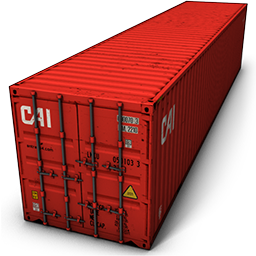
\includegraphics[height=4cm]{images/container.png}
	\end{center}
\end{frame}

\begin{frame}{I contenitori}
	Qt offre una nutrita serie di contenitori che permettono di soddisfare le esigenze più comuni.
	\bigskip
	\begin{columns}
		\column{0.85\textwidth}
		\begin{block}{}
			{\ttfamily QList<T>}: array di puntatori, accesso via indice rapido\\
			{\ttfamily QLinkedList<T>}: lista concatenata, inserimenti rapidi\\
			{\ttfamily QVector<T>}: array vero e proprio, inserimenti lenti\\
			{\ttfamily QStack<T>}: pila LIFO, basato su {\ttfamily QVector<T>}\\
			{\ttfamily QQueue<T>}: coda FIFO, basato su {\ttfamily QList<T>}\\
			{\ttfamily QSet<T>}: senza ordinato né duplicati, basato su {\ttfamily QHash}
		\end{block}
	\end{columns}
	\bigskip
\end{frame}

\begin{frame}{I contenitori (esempio)}
	Hanno interfacce abbastanza simili
	\bigskip
	\begin{columns}
		\column{0.5\textwidth}
		\begin{block}{}
			{\ttfamily QList<QString> lista;\\
				lista.append("primo");\\
				lista += "secondo";\\
				lista.push\_back("terzo");\\
				lista.removeLast();}
		\end{block}
	\end{columns}
	\bigskip
\end{frame}

\begin{frame}{Contenitori chiave-valore}
	Qt offre una nutrita serie di contenitori che permettono di soddisfare le esigenze più comuni.
	\bigskip
	\begin{columns}
		\column{0.8\textwidth}
		\begin{block}{}
			{\ttfamily QMap<Key,T>}: array associativo ordinato per chiave\\
			{\ttfamily QMultiMap<Key,T>}: più di un valore per chiave\\
			{\ttfamily QHash<Key,T>}: non ordinato, lookup rapidi\\
			{\ttfamily QMultiHash<Key,T>}
		\end{block}
	\end{columns}
\end{frame}

\begin{frame}{I contenitori chiave-valore (esempio)}
Hanno interfacce abbastanza simili
\bigskip
\begin{columns}
	\column{0.75\textwidth}
	\begin{block}{}
		{\ttfamily QHash<QString, int> punteggio;\\
			punteggio.insert("Andrea", 1);\\
			punteggio.insert("Paolo", 3);\\
			punteggio.insert("Franco", 0);\\
			std::cout << punteggio["Franco"] << std::endl;}
	\end{block}
\end{columns}
\end{frame}

\begin{frame}{Il modello ad oggetti di Qt}
	Qt si basa sul \textbf{Qt object model}. E' questa architettura a rendere Qt potente e facile da usare. Il tutto si basa sulla classe {\ttfamily QObject} e sul tool {\ttfamily moc}.
	
	Facendo derivare tutte le classi dalla classe {\ttfamily QObject}, si ottengono una serie di vantaggi. Eccoli elencati qui:
	
	\begin{itemize}
		\item Gestione semplificata della memoria
		\item Segnali e slot
		\item Introspezione
	\end{itemize}
\end{frame}

\begin{frame}{Gestione semplificata della memoria}
	Quando si crea un'istanza di una classe derivata da {\ttfamily QObject}, è possibile passare al costruttore un puntatore a un oggetto padre. Questa è la base della gestione semplificata della memoria.
	
	\bigskip
	Quando un padre viene cancellato (ossia si esegue una {\ttfamily delete} su di esso), vengono cancellati anche tutti i suoi figli. Ciò significa che una classe derivata da {\ttfamily QObject} può creare istanze di figli di {\ttfamily QObject} passando {\ttfamily this} come padre senza preoccuparsi della loro distruzione.
\end{frame}

\begin{frame}{Gestione semplificata della memoria (esempio)}
	\begin{columns}
		\column{0.45\textwidth}
		\begin{block}{}
			\centering
			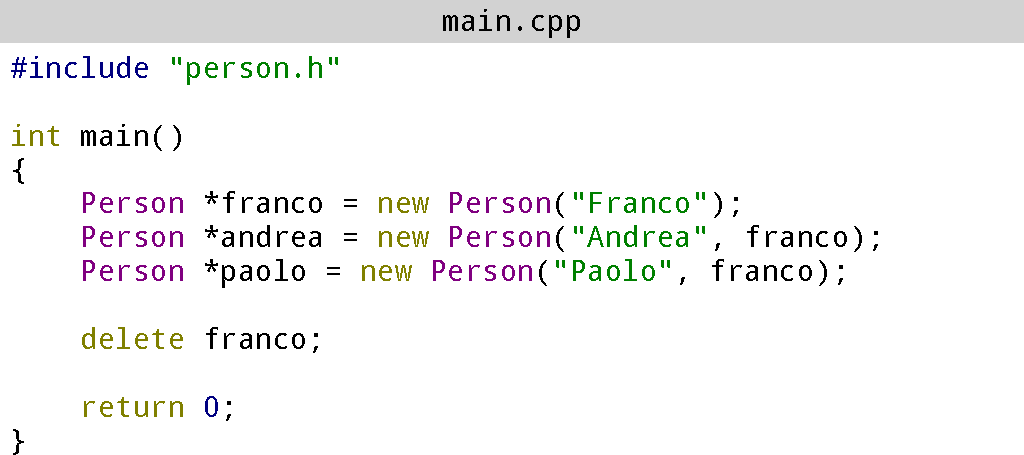
\includegraphics[width=\textwidth]{images/es1main.pdf}
		\end{block}
		\column{0.45\textwidth}
		\begin{block}{}
			\centering
			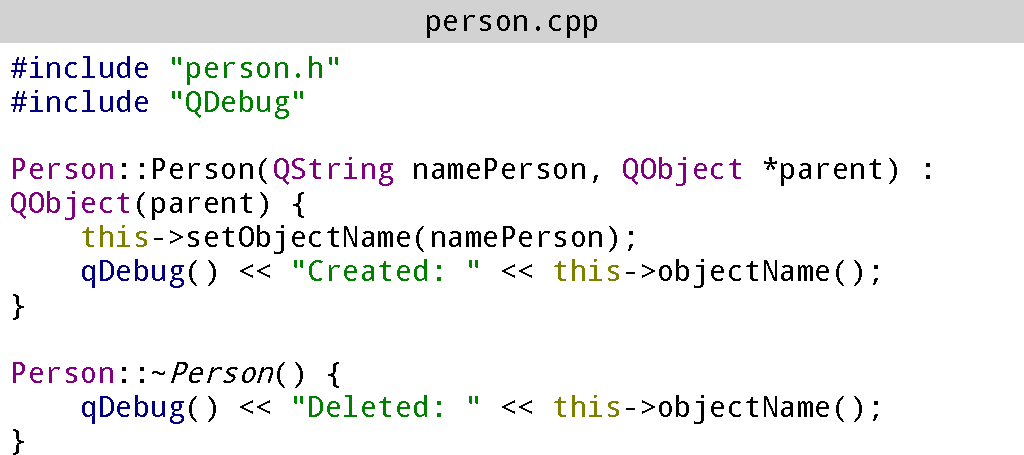
\includegraphics[width=\textwidth]{images/es1person.pdf}
		\end{block}
	\end{columns}
	\begin{columns}
		\column{0.5\textwidth}
		\begin{block}{}\tiny
			{\ttfamily \$ qmake \&\& make \&\& ./qobject-sample\\
				Created:  "Franco"\\
				Created:  "Andrea"\\
				Created:  "Paolo"\\
				Deleted:  "Franco"\\
				Deleted:  "Andrea"\\
				Deleted:  "Paolo"\\
			}
		\end{block}
	\end{columns}
	\bigskip
	Come si può vedere, tutti gli oggetti vengono cancellati, prima i genitori e poi i figli.
\end{frame}

\begin{frame}{Compilazione ed esecuzione di un applicativo}
	La sequenza di comandi (comunemente detti ``tool'') che vengono attivati per passare dal file {\ttfamily qobject-sample.pro} al file eseguibile {\ttfamily ./qobject-sample} è detta ``toolchain''.
	
	Quando facciamo il ``Build'' del programma vengono eseguiti i seguenti ``tool'' della libreria Qt:
	\begin{enumerate}
		\item {\ttfamily qmake}, converte il file progetto nel {\ttfamily MakeFile}
		\item {\ttfamily make}, interpreta il {\ttfamily MakeFile}
		\item {\ttfamily moc}, genera il codice di supporto per i Qt Meta Objects
		\item {\ttfamily rcc}, converte il file delle risorse in file {\ttfamily C++}
		\item {\ttfamily uic}, converte i file {\ttfamily .ui} in file {\ttfamily C++}
	\end{enumerate}
\end{frame}


\begin{frame}{Segnali e slot}
	\begin{columns}
		\column{0.35\textwidth}
		\begin{figure}
			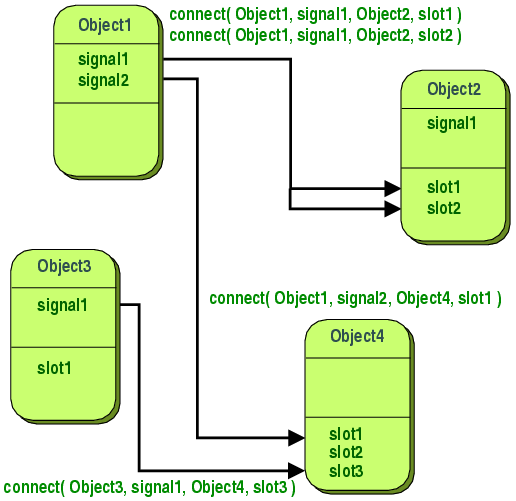
\includegraphics[width=\textwidth]{images/signal-slot.png}
		\end{figure}
		\column{0.60\textwidth}
		\begin{block}{}
			Segnali (\textit{sig}nals) e slot (\textit{slots}) permettono di legare insieme due oggetti senza che nessuno dei due sappia nulla dell'altro. 
			
			\bigskip
			È possibile, ad esempio, costruire due classi {\ttfamily A} e {\ttfamily B} e fare in modo che ad un evento di {\ttfamily A} corrisponda un azione di {\ttfamily B} e viceversa senza doversi minimamente preoccupare di inserire in {\ttfamily A} riferimenti di {\ttfamily B}.
		\end{block}
	\end{columns}
\end{frame}

\begin{frame}{Segnali e slot}
	\begin{columns}
		\column{0.35\textwidth}
		\begin{figure}
			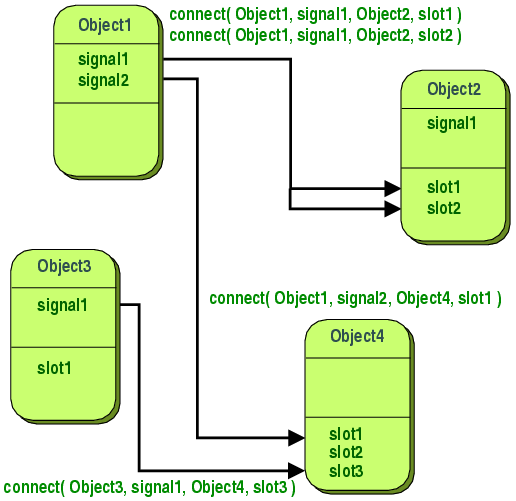
\includegraphics[width=\textwidth]{images/signal-slot.png}
		\end{figure}
		\column{0.60\textwidth}
		\begin{block}{}
			Un \textit{segnale} è un avviso emesso da un oggetto al verificarsi di determinate condizioni. Ad ogni \textit{segnale} è collegato uno \textit{slot} ovvero una funzione {\ttfamily C/C++}.
		\end{block}	
		\bigskip	
		\begin{block}{}
			Per collegare un segnale ad uno slot si usa il comando:
			\begin{center}
				\footnotesize
				{\ttfamily connect(sender, SIGNAL(signal), receiver, SLOT(slot));}
			\end{center}
		\end{block}
	\end{columns}
\end{frame}

\begin{frame}{Segnali e slot}
	\begin{block}{}
		\begin{center}
			{\ttfamily connect(sender, SIGNAL(signal), receiver, SLOT(slot));}
		\end{center}
	\end{block}
	\bigskip
	Possiamo avere varie forme di connessioni:
	\begin{itemize}
		\item \textbf{Più segnali collegati ad un solo slot}: la stessa funzione viene lanciata in corrispondenza di due o più segnali differenti.
		\item \textbf{Un solo segnale collegato a più slot}: l'arrivo di un segnale genera l'esecuzione di più funzioni. Tali funzioni vengono eseguite una dopo l'altra in un ordine indefinito.
		\item \textbf{Un segnale collegato a un segnale}: l'arrivo di un segnale causa semplicemente il lancio di un nuovo segnale.
	\end{itemize}
\end{frame}

\begin{frame}{Segnali e slot}
	\begin{block}{Connessioni automatiche}
		A volte si hanno molti segnali e slot da collegare. Usando delle convenzioni si può ottenere un collegamento automatico. 
		
		Questo si realizza con {\ttfamily QMetaObject::connectSlotsByName}
		\begin{itemize}
			\item tutti gli oggetti figli (children) dell'oggetto
			\item il nome e i segnali di ciascun figlio
		\end{itemize}
		
		\bigskip
		Associa i segnali dei figli allo slot corrispondente:
		
		\bigskip
		\centering
		{\ttfamily \textcolor{blue}{void} on\_<\textcolor{purple}{nome\_figlio}>\_<\textcolor{purple}{nome\_segnale}>(<parametri>)}
	\end{block}
\end{frame}

\begin{frame}{L'introspezione}
	\begin{block}{}
		L'introspezione\footnote{altresì nota come reflection} è la capacità di un programma di eseguire elaborazioni che hanno per oggetto il programma stesso, e in particolare la struttura del suo codice sorgente.
	\end{block}	
	
	\begin{itemize}
		\item È un’alternativa all'introspezione di C++ (RTTI)
		\item {\ttfamily QObject} offre informazioni sulla struttura di una classe:
		\begin{itemize}
			\item Nome della classe
			\item Classe da cui eredita
			\item Metodi e costruttori
			\item Segnali, slot e proprietà
		\end{itemize}
		\item Si richiama tramite il metodo {\ttfamily QObject::metaObject()}\footnote{\url{http://doc.qt.io/qt-5/qobject.html\#metaObject}}
	\end{itemize}
\end{frame}

\defverbatim[colored]\lst{%
\begin{lstlisting}[tabsize=4,basicstyle=\ttfamily]
TestClass istanza(NULL);
const QMetaObject *instanza_info = instanza.metaObject();

cout << instanza_info->className() << endl;
for (int i = 0; i < istanza_info->methodCount(); i++)
	cout << istanza_info->method(i).signature() << endl;
\end{lstlisting}
}

\begin{frame}{L'introspezione (esempio)}
	\begin{block}{}
		\lst
	\end{block}
\end{frame}

\begin{frame}{Threading in Qt}
	\begin{block}{}
		Un thread o thread di esecuzione, in informatica, è una suddivisione di un processo in due o più filoni o sottoprocessi, che vengono eseguiti concorrentemente da un sistema di elaborazione monoprocessore (multithreading) o multiprocessore o Multicore.
	\end{block}
	\bigskip
	Qt offre vari metodi per l'esecuzione parallela di codice:
	\begin{itemize}
		\item {\ttfamily QThread}
		\item {\ttfamily QSemaphore}
		\item \dots
	\end{itemize}
	
\end{frame}

\begin{frame}{QThread}
	Per creare un thread è sufficiente ereditare da {\ttfamily QThread}. Il suo metodo principale è {\ttfamily QThread::run()}.\\
	\bigskip
	
	\begin{center}
		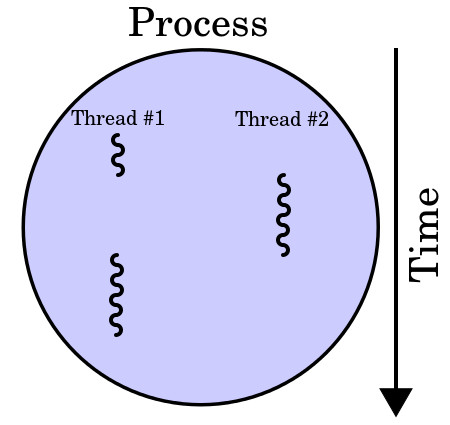
\includegraphics[height=3cm]{images/multithread.jpg}
	\end{center}
	
	Per lanciare un thread si usa {\ttfamily QThread::start()}, mentre  {\ttfamily QThread::wait()} permette di attendere la terminazione.
\end{frame}

\defverbatim[colored]\lst{%
	\begin{lstlisting}[tabsize=4,basicstyle=\ttfamily]

	\end{lstlisting}
}

\begin{frame}{QSemaphore}
	È un semplice meccanismo di sincronizzazione a semaforo.\\
	Alla creazione fissiamo il numero di thread concorrenti
	\begin{columns}
		\column{0.7\textwidth}
		\begin{block}{}
			{\ttfamily QSemaphore semaforo(1);\\
				semaforo.acquire();\\
				// Qui l'esecuzione sara' possibile\\
				// solo un thread alla volta\\
				semaforo.release();}
		\end{block}
	\end{columns}
	
\end{frame}


\begin{frame}{Una prima applicazione grafica}
	\begin{figure}
		
\includegraphics[height=5cm]{images/coding.jpg}
	\end{figure}
\end{frame}

\begin{frame}{\,}
	\begin{center}
		
\includegraphics[height=5cm]{images/thats-all-folks.jpg}
	\end{center}
	\begin{block}{}
		Special thanks to POuL - Politecnico Open unix Labs
	\end{block}
	
\end{frame}
\end{document}
